\subsection{Pegeldiagram}
\label{sec:Pegeldiagram}

Nachfolgend ist in der Abbildung \ref{pic:Pegeldiagram_Line} das Pegeldiagramm des Signalpfades dargestellt.
Von Line IN können Signale mit bis zu $2 \si{V_{RMS}}$ bzw. $+6 \si{dBV}$ ankommen. Mit einem 1/2 Spannungsteiler wird das Signal um $6 \si{dB}$ abgeschwächt.
Der Codec hat eine maximale Dynamic Range von $90 \si{dB}$ und einen maximalen Ausgangspegel von $1 \si{V_{RMS}}$ bzw. $0 \si{dBV}$.

\begin{figure}[H]
	\centering
	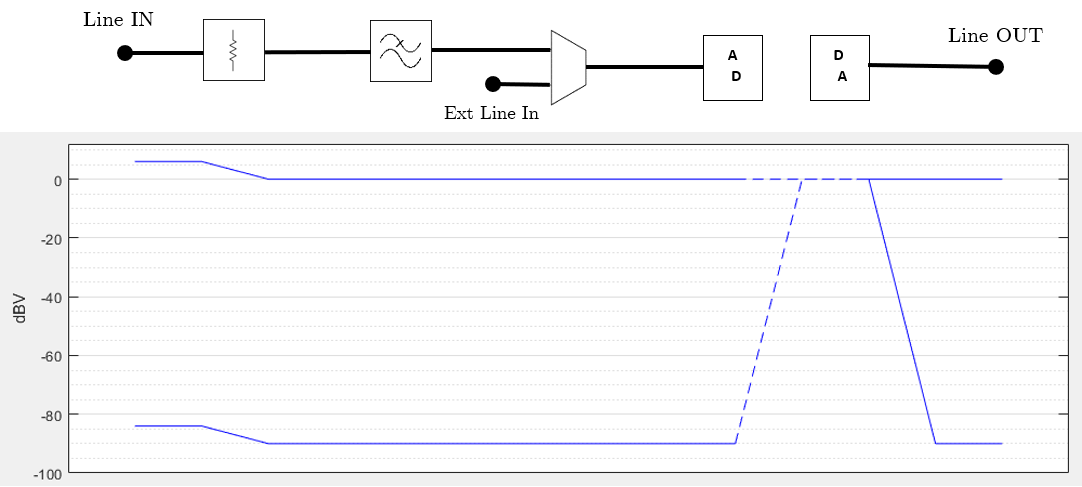
\includegraphics[width=1.0\linewidth]{level_diagram_line}
	\caption{Pegeldiagram des Audiopfades von Line IN nach Line OUT}
	\label{pic:Pegeldiagram_Line}
\end{figure}

